\par
\section{Driver programs found in the {\tt Misc} directory}
\label{section:Misc:drivers}
\par
This section contains brief descriptions of the driver programs.
\par
%=======================================================================
\begin{enumerate}
%-----------------------------------------------------------------------
\item
\begin{verbatim}
testNDperm msglvl msgFile n1 n2 n3 outPermFile
\end{verbatim}
This driver program generates a {\tt Perm} object that contains a
nested dissection ordering for a {\tt n1 x n2 x n3} regular grid.
\par
\begin{itemize}
\item
The {\tt msglvl} parameter determines the amount of output ---
taking {\tt msglvl >= 3} means the {\tt Perm} object is written
to the output file.
\item
The {\tt msgFile} parameter determines the message file --- if {\tt
msgFile} is {\tt stdout}, then the message file is {\it stdout},
otherwise a file is opened with {\it append} status to receive any
output data.
\item
{\tt n1} is the number of points in the first direction.
\item
{\tt n2} is the number of points in the second direction.
\item
{\tt n3} is the number of points in the third direction.
\item
The {\tt outPermFile} parameter is the output file for the {\tt Perm}
object. 
If {\tt outPermFile} is {\tt none} then the {\tt Perm} object is not
written to a file. 
Otherwise, the {\tt Perm\_writeToFile()} method is called to write
the object to 
a formatted file (if {\tt outPermFile} is of the form {\tt *.permf}),
or
a binary file (if {\tt outPermFile} is of the form {\tt *.permb}).
\end{itemize}
%-----------------------------------------------------------------------
\item
\begin{verbatim}
testOrderViaMMD msglvl msgFile GraphFile seed ETreeFile
\end{verbatim}
This program reads in a {\tt Graph} object from a file and computes
a multiple minimum degree ordering of the graph.
\par
\begin{itemize}
\item
The {\tt msglvl} parameter determines the amount of output ---
taking {\tt msglvl >= 3} means the {\tt Perm} object is written
to the output file.
\item
The {\tt msgFile} parameter determines the message file --- if {\tt
msgFile} is {\tt stdout}, then the message file is {\it stdout},
otherwise a file is opened with {\it append} status to receive any
output data.
\item
The {\tt inGraphFile} parameter is the input file for the {\tt Graph}
object. It must be of the form {\tt *.graphf} or {\tt *.graphb}.
The {\tt Graph} object is read from the file via the
{\tt Graph\_readFromFile()} method.
\item
The {\tt seed} parameter is a random number seed.
\item
The {\tt ETreeFile} parameter is the output file for the {\tt ETree}
object. 
If {\tt ETreeFile} is {\tt none} then the {\tt ETree} object is not
written to a file. 
Otherwise, the {\tt ETree\_writeToFile()} method is called to write
the object to 
a formatted file (if {\tt ETreeFile} is of the form {\tt *.etreef}),
or
a binary file (if {\tt ETreeFile} is of the form {\tt *.etreeb}).
\end{itemize}
%-----------------------------------------------------------------------
\item
\begin{verbatim}
testOrderViaND msglvl msgFile GraphFile maxdomainsize seed ETreeFile
\end{verbatim}
This program reads in a {\tt Graph} object from a file and computes
a generalized nested dissection ordering of the graph.
\par
\begin{itemize}
\item
The {\tt msglvl} parameter determines the amount of output ---
taking {\tt msglvl >= 3} means the {\tt Perm} object is written
to the output file.
\item
The {\tt msgFile} parameter determines the message file --- if {\tt
msgFile} is {\tt stdout}, then the message file is {\it stdout},
otherwise a file is opened with {\it append} status to receive any
output data.
\item
The {\tt inGraphFile} parameter is the input file for the {\tt Graph}
object. It must be of the form {\tt *.graphf} or {\tt *.graphb}.
The {\tt Graph} object is read from the file via the
{\tt Graph\_readFromFile()} method.
\item
The {\tt maxdomainsize} parameter governs the partition of a graph.
If a subgraph has more than {\tt maxdomainsize} vertices, it is
split.
\item
The {\tt seed} parameter is a random number seed.
\item
The {\tt ETreeFile} parameter is the output file for the {\tt ETree}
object. 
If {\tt ETreeFile} is {\tt none} then the {\tt ETree} object is not
written to a file. 
Otherwise, the {\tt ETree\_writeToFile()} method is called to write
the object to 
a formatted file (if {\tt ETreeFile} is of the form {\tt *.etreef}),
or
a binary file (if {\tt ETreeFile} is of the form {\tt *.etreeb}).
\end{itemize}
%-----------------------------------------------------------------------
\item
\begin{verbatim}
testOrderViaMS msglvl msgFile GraphFile maxdomainsize seed ETreeFile
\end{verbatim}
This program reads in a {\tt Graph} object from a file and computes
a multisection ordering of the graph.
\par
\begin{itemize}
\item
The {\tt msglvl} parameter determines the amount of output ---
taking {\tt msglvl >= 3} means the {\tt Perm} object is written
to the output file.
\item
The {\tt msgFile} parameter determines the message file --- if {\tt
msgFile} is {\tt stdout}, then the message file is {\it stdout},
otherwise a file is opened with {\it append} status to receive any
output data.
\item
The {\tt inGraphFile} parameter is the input file for the {\tt Graph}
object. It must be of the form {\tt *.graphf} or {\tt *.graphb}.
The {\tt Graph} object is read from the file via the
{\tt Graph\_readFromFile()} method.
\item
The {\tt maxdomainsize} parameter governs the partition of a graph.
If a subgraph has more than {\tt maxdomainsize} vertices, it is
split.
\item
The {\tt seed} parameter is a random number seed.
\item
The {\tt ETreeFile} parameter is the output file for the {\tt ETree}
object. 
If {\tt ETreeFile} is {\tt none} then the {\tt ETree} object is not
written to a file. 
Otherwise, the {\tt ETree\_writeToFile()} method is called to write
the object to 
a formatted file (if {\tt ETreeFile} is of the form {\tt *.etreef}),
or
a binary file (if {\tt ETreeFile} is of the form {\tt *.etreeb}).
\end{itemize}
%-----------------------------------------------------------------------
\item
\begin{verbatim}
drawGraph msglvl msgFile inGraphFile inCoordsFile inTagsIVfile
          outEPSfile linewidth1 linewidth2 bbox[4] rect[4] radius
\end{verbatim}
This driver program generates a Encapsulated Postscript file 
{\tt outEPSfile} of a 2-D graph using a {\tt Graph} object,
a {\tt Coords} object and a tags {\tt IV} object that contains the
component ids of the vertices.
\par
See the {\tt doDraw} script file in this directory for an example
calling sequence.
\begin{itemize}
\item
The {\tt msglvl} parameter determines the amount of output ---
taking {\tt msglvl >= 3} means that all objects are written
to the output file.
\item
The {\tt msgFile} parameter determines the message file --- if {\tt
msgFile} is {\tt stdout}, then the message file is {\it stdout},
otherwise a file is opened with {\it append} status to receive any
output data.
\item
The {\tt inGraphFile} parameter is the input file for the {\tt Graph}
object. It must be of the form {\tt *.graphf} or {\tt *.graphb}.
The {\tt Graph} object is read from the file via the
{\tt Graph\_readFromFile()} method.
\item
The {\tt inCoordsFile} parameter is the input file for the {\tt Coords}
object. It must be of the form {\tt *.coordsf} or {\tt *.coordsb}.
The {\tt Coords} object is read from the file via the
{\tt Coords\_readFromFile()} method.
\item
The {\tt inTagsIVfile} parameter is the input file for the tags
{\tt IV} object. 
It must be of the form {\tt 'none'}, {\tt *.ivf} or {\tt *.ivb}.
The {\tt IV} object is read from the file via the
{\tt IV\_readFromFile()} method.
\item
The {\tt outEPSfile} parameter is the output file for the Encapsulated
Postscript file.
\item
The {\tt linewidth1} parameter governs the linewidth of edges
between vertices in the same component.
\item
The {\tt linewidth2} parameter governs the linewidth of edges
between vertices in different components.
\item
The {\tt bbox[4]} array is the bounding box for the plot.
In Postscript the coordinates are in {\it points}, where there are
72 points per inch.
For example, a bounding box of {\tt 0 0 200 300} will create a plot
whose size is 2.78 inches by 4.17 inches.
\item
The {\tt rect[4]} array is the enclosing rectangle for the plot.
To put a 20 point margin around the plot, set
{\tt rect[0] = bbox[0] + 20},
{\tt rect[1] = bbox[1] + 20},
{\tt rect[2] = bbox[2] - 20} and
{\tt rect[3] = bbox[3] - 20}.
\item
The {\tt radius} parameter governs the size of the filled circle
that is centered on each vertex.
The dimension is in points.
\end{itemize}
See Figure~\ref{fig-R2D100} for a plot of the graph of {\tt R2D100},
a randomly triangulated grid with 100 vertices with {\tt linewidth1
= 3}.
Figure~\ref{fig-R2D100-fishnet} illustrates a domain decomposition
obtained from the fishnet algorithm 
of Chapter~\ref{chapter:GPart:intro} 
with {\tt linewidth1 = 3} and {\tt linewidth2 = 0.1}.
\par
\begin{figure}[htbp]
\caption{{\sc R2D100}}
\label{fig-R2D100}
\begin{center}
\mbox{
% \psfig{file=R2D100notags.eps,height=4.00in,width=4.00in}
\psfig{file=../../misc/doc/R2D100notags.eps,height=4.00in,width=4.00in}
}
\end{center}
\end{figure}
\par
\begin{figure}[htbp]
\caption{{\sc R2D100: fishnet domain decomposition}}
\label{fig-R2D100-fishnet}
\begin{center}
\mbox{
% \psfig{file=R2D100fishnet.eps,height=4.00in,width=4.00in}
\psfig{file=../../misc/doc/R2D100fishnet.eps,height=4.00in,width=4.00in}
}
\end{center}
\end{figure}

%-----------------------------------------------------------------------
\item
\begin{verbatim}
testSemi msglvl msgFile GraphFile ETreeFile mapFile
\end{verbatim}
This program is used to compute the effect of using a semi-implicit
factorization to solve 
$$
AX = 
\left \lbrack \begin{array}{cc}
A_{0,0} & A_{0,1} \cr
A_{1,0} & A_{1,1} 
\end{array} \right \rbrack
\left \lbrack \begin{array}{c}
X_0 \cr
X_1 
\end{array} \right \rbrack
=
\left \lbrack \begin{array}{c}
B_0 \cr
B_1 
\end{array} \right \rbrack
= B.
$$
$A$ is factored as
$$
\left \lbrack \begin{array}{cc}
A_{0,0} & A_{0,1} \cr
A_{1,0} & A_{1,1} 
\end{array} \right \rbrack
=
\left \lbrack \begin{array}{cc}
L_{0,0} & 0 \cr
L_{1,0} & L_{1,1} 
\end{array} \right \rbrack
\left \lbrack \begin{array}{cc}
U_{0,0} & U_{0,1} \cr
 0 & U_{1,1} 
\end{array} \right \rbrack,
$$
and to solve $AX = B$, we do the following steps.
\begin{itemize}
\item solve $L_{0,0} Y_0 = B_0$
\item solve $L_{1,1} U_{1,1} X_1 = B_1 - L_{1,0} Y_0$
\item solve $U_{0,0} X_0 = Y_0 - U_{0,1} X_1$
\end{itemize}
An alternative factorization is
$$
A =
\left \lbrack \begin{array}{cc}
L_{0,0} & 0 \cr
A_{1,0}U_{0,0}^{-1} & L_{1,1} 
\end{array} \right \rbrack
\left \lbrack \begin{array}{cc}
U_{0,0} & L_{0,0}^{-1}U_{0,1} \cr
 0 & U_{1,1} 
\end{array} \right \rbrack.
$$
To solve $AX = B$, we do the following {\it semi-implicit solve}.
\begin{itemize}
\item solve $L_{0,0} U_{0,0} Z_0 = B_0$
\item solve $L_{1,1} U_{1,1} X_1 = B_1 - A_{1,0} Z_0$
\item solve $L_{0,0} U_{0,0} X_0 = B_0 - A_{0,1} X_1$
\end{itemize}
When we compare the semi-implicit solve against the explicit solve,
we see that the former needs
$A_{0,1}$ and $A_{1,0}$ but not $L_{1,0}$ or $A_{0,1}$.
and executes two solves with $L_{0,0}$ and $U_{0,0}$ (instead of one)
and performs a matrix-matrix multiply with $A_{0,1}$ and $A_{1,0}$
instead of $L_{1,0}$ and $U_{0,1}$.
In situations where the numbers of entries in $L_{1,0}$ and
$U_{0,1}$ are much larger than those in $A_{1,0}$ and $A_{0,1}$,
and the numbers of entries in $L_{0,0}$ and $U_{0,0}$ are not too
large, the semi-implicit factorization can be more efficient.
\par
This program reads in three objects:
a {\tt Graph} object,
an {\tt ETree} object to specify the ordering,
and an {\tt IV} map object that tells which vertices are in the
which blocks of the matrix.
The map from vertices to blocks follows the same convention as the
{\it component map} from the {\tt GPart} object.
If {\tt map[v] = 0}, then vertex {\tt v} belongs to the Schur
complement $(1,1)$ block.
Otherwise, {\tt v} belongs to a domain (the domain number is {\tt
map[v]}) and so belongs to the $(0,0)$ block.
The output of the program gives statistics for storage and
operation count for the two types of solves.
For example,
\begin{verbatim}
 storage: explicit = 1404, semi-implicit = 1063, ratio = 1.321
 opcount: explicit = 2808, semi-implicit = 2742, ratio = 1.024
\end{verbatim}
is the output using the {\tt do\_testSemi} driver program for
the {\tt R2D100} matrix.
\par
\begin{itemize}
\item
The {\tt msglvl} parameter determines the amount of output.
\item
The {\tt msgFile} parameter determines the message file --- if {\tt
msgFile} is {\tt stdout}, then the message file is {\it stdout},
otherwise a file is opened with {\it append} status to receive any
output data.
\item
The {\tt GraphFile} parameter is the input file for the {\tt Graph}
object. It must be of the form {\tt *.graphf} or {\tt *.graphb}.
The {\tt Graph} object is read from the file via the
{\tt Graph\_readFromFile()} method.
\item
The {\tt ETreeFile} parameter is the input file for the {\tt ETree}
object. It must be of the form {\tt *.etreef} or {\tt *.etreeb}.
The {\tt ETree} object is read from the file via the
{\tt ETree\_readFromFile()} method.
\item
The {\tt mapFile} parameter is the input file for the map {\tt IV}
object. It must be of the form {\tt *.ivf} or {\tt *.ivb}.
The {\tt IV} object is read from the file via the
{\tt IV\_readFromFile()} method.
\end{itemize}
%-----------------------------------------------------------------------
\item
\begin{verbatim}
allInOne msglvl msgFile type symmetryflag pivotingflag
         matrixFileName rhsFileName seed
\end{verbatim}
This {\it all-in-one} driver program is an example that tests the
serial $U^TDU$, $U^HDU$ or $LU$ factorization and solve.
Matrix entries are read in from a file, and then the matrix 
is assembled and factored.
The right hand side entries are read in from a file, and the system
is solved.
Three input parameters specify the type of system (real or
complex),
the type of factorization (symmetric, Hermitian or nonsymmetric)
and whether pivoting is to be used for numerical stability.
\par
\begin{itemize}
\item
The {\tt msglvl} parameter determines the amount of output ---
taking {\tt msglvl >= 3} means the {\tt Perm} object is written
to the output file.
\item
The {\tt msgFile} parameter determines the message file --- if {\tt
msgFile} is {\tt stdout}, then the message file is {\it stdout},
otherwise a file is opened with {\it append} status to receive any
output data.
\item
{\tt type} is the type of entries
\begin{itemize}
\item {\tt 1} --- ({\tt SPOOLES\_REAL}) for real entries
\item {\tt 2} --- ({\tt SPOOLES\_COMPLEX}) for complex entries
\end{itemize}
\item
{\tt symmetryflag} defines the factorization
\begin{itemize}
\item {\tt 0} --- ({\tt SPOOLES\_SYMMETRIC}) 
for a real or complex $U^TDU$ factorization
\item {\tt 1} --- ({\tt SPOOLES\_SYMMETRIC}) 
for a complex $U^HDU$ factorization
\item {\tt 2} --- ({\tt SPOOLES\_SYMMETRIC}) 
for a real or complex $LU$ factorization
\end{itemize}
\item
{\tt pivotingflag} defines pivoting or not for numerical stability
\begin{itemize}
\item {\tt 0} --- ({\tt SPOOLES\_NO\_PIVOTING}) for no pivoting
\item {\tt 1} --- ({\tt SPOOLES\_PIVOTING}) for pivoting
\end{itemize}
Note, the code has a pivoting threshold {\tt tau = 100} hardwired
into the code.
\item
The {\tt matrixFileName} parameter is the name of the input file
for the matrix entries.
For a real matrix, this file must have the following form.
\begin{verbatim}
nrow ncol nent
...
irow jcol value
...
\end{verbatim}
where the first line has the number of rows, columns and entries.
(Note, for this driver program {\tt nrow} must be equal to {\tt ncol}
since we are factoring a square matrix.)
Each of the {\tt nent} following lines contain one nonzero entry.
For a complex matrix, the file has this structure.
\begin{verbatim}
nrow ncol nent
...
irow jcol real_value imag_value
...
\end{verbatim}
For both real and complex entries, the entries need not be
disjoint,
i.e., entries with the same {\tt irow} and {\tt jcol} values are
{\it summed}.
\item
The {\tt rhsFileName} parameter is the name of the input file for
the right hand side matrix.
It has the following structure
\begin{verbatim}
nrow nrhs
...
irow value_0 value_1 ... value_\{nrhs-1\}
...
\end{verbatim}
Note, {\tt nrow} need not be the number of equations, here it is
the number of nonzero right hand side entries.
This allows us to input sparse right hand sides without specifying
the zeroes.
In contrast to the input for the matrix entries, the nonzero rows
{\it must} be unique.
The right hand side entries are not assembled into a dense matrix
object, but placed into the object.
\item
{\tt seed} is a random number seed used for the ordering process.
\end{itemize}
%-----------------------------------------------------------------------
\item
\begin{verbatim}
patchAndGo msglvl msgFile type symmetryflag patchAndGoFlag fudge toosmall

           storeids storevalues matrixFileName rhsFileName seed 
\end{verbatim}
This driver program is used to test the ``patch-and-go''
functionality for a factorization without pivoting.
When small diagonal pivot elements are found, 
one of three actions are taken.
See the {\tt PatchAndGoInfo} object for more information.
\par
The program reads in a matrix $A$ and right hand side $B$,
generates the graph for $A$ and orders the matrix,
factors $A$ and solves the linear system $AX = B$ for $X$
using multithreaded factors and solves.
Use the script file {\tt do\_patchAndGo} for testing.
\par
\begin{itemize}
\item
The {\tt msglvl} parameter determines the amount of output.
Use {\tt msglvl = 1} for just timing output.
\item
The {\tt msgFile} parameter determines the message file --- if {\tt
msgFile} is {\tt stdout}, then the message file is {\it stdout},
otherwise a file is opened with {\it append} status to receive any
output data.
\item
The {\tt type} parameter specifies a real or complex linear system.
\begin{itemize}
\item
{\tt type = 1 (SPOOLES\_REAL)} for real,
\item
{\tt type = 2 (SPOOLES\_COMPLEX)} for complex.
\end{itemize}
\item
The {\tt symmetryflag} parameter specifies the symmetry of the matrix.
\begin{itemize}
\item
{\tt type = 0 (SPOOLES\_SYMMETRIC)} for $A$ real or complex symmetric,
\item
{\tt type = 1 (SPOOLES\_HERMITIAN)} for $A$ complex Hermitian,
\item
{\tt type = 2 (SPOOLES\_NONSYMMETRIC)}
\end{itemize}
for $A$ real or complex nonsymmetric.
\item
The {\tt patchAndGoFlag} specifies the ``patch-and-go'' strategy.
\begin{itemize}
\item
{\tt patchAndGoFlag = 0} --- if a zero pivot is detected, stop
computing the factorization, set the error flag and return.
\item
{\tt patchAndGoFlag = 1} --- if a small or zero pivot is detected,
set the diagonal entry to 1 and the offdiagonal entries to zero.
\item
{\tt patchAndGoFlag = 2} --- if a small or zero pivot is detected,
perturb the diagonal entry.
\end{itemize}
\item
The {\tt fudge} parameter is used to perturb a diagonal entry.
\item
The {\tt toosmall} parameter is judge when a diagonal entry is small.
\item
If {\tt storeids = 1}, then the locations where action was taken is
stored in an {\tt IV} object.
\item
If {\tt storevalues = 1}, then the perturbations are
stored in an {\tt DV} object.
\item
The {\tt matrixFileName} parameter is the name of the files where
the matrix entries are read from.
The file has the following structure.
\begin{verbatim}
neqns neqns nent
irow jcol entry
...  ...  ...
\end{verbatim}
where {\tt neqns} is the global number of equations and {\tt nent}
is the number of entries in this file.
There follows {\tt nent} lines, each containing a row index, a
column index and one or two floating point numbers, one if real,
two if complex.
\item
The {\tt rhsFileName} parameter is the name of the files where
the right hand side entries are read from.
The file has the following structure.
\begin{verbatim}
nrow nrhs
irow entry ... entry
...  ...   ... ...
\end{verbatim}
where {\tt nrow} is the number of rows in this file
and {\tt nrhs} is the number of rigght and sides.
There follows {\tt nrow} lines, each containing a row index
and either {\tt nrhs} or {\tt 2*nrhs} floating point numbers,
the first if real, the second if complex.
\item
The {\tt seed} parameter is a random number seed.
\end{itemize}
%-----------------------------------------------------------------------
\item
\begin{verbatim}
QRallInOne msglvl msgFile type matrixFileName rhsFileName seed
\end{verbatim}
This {\it all-in-one} driver program is an example that tests the
serial $QR$ factorization and solve.
Matrix entries are read in from a file, and then the matrix 
is assembled and factored.
The right hand side entries are read in from a file, and the system
is solved.
One input parameter specifies the type of system (real or
complex).  
\par
\begin{itemize}
\item
The {\tt msglvl} parameter determines the amount of output ---
taking {\tt msglvl >= 3} means the {\tt Perm} object is written
to the output file.
\item
The {\tt msgFile} parameter determines the message file --- if {\tt
msgFile} is {\tt stdout}, then the message file is {\it stdout},
otherwise a file is opened with {\it append} status to receive any
output data.
\item
{\tt type} is the type of entries
\begin{itemize}
\item {\tt 1} --- ({\tt SPOOLES\_REAL}) for real entries
\item {\tt 2} --- ({\tt SPOOLES\_COMPLEX}) for complex entries
\end{itemize}
\item
The {\tt matrixFileName} parameter is the name of the input file
for the matrix entries.
For a real matrix, this file must have the following form.
\begin{verbatim}
nrow ncol nent
...
irow jcol value
...
\end{verbatim}
where the first line has the number of rows, columns and entries.
Each of the {\tt nent} following lines contain one nonzero entry.
For a complex matrix, the file has this structure.
\begin{verbatim}
nrow nrhs nent
...
irow jcol real_value imag_value
...
\end{verbatim}
For both real and complex entries, the entries need not be
disjoint,
i.e., entries with the same {\tt irow} and {\tt jcol} values are
{\it summed}.
\item
The {\tt rhsFileName} parameter is the name of the input file for
the right hand side matrix.
It has the following structure
\begin{verbatim}
nrow nrhs
...
irow value_0 value_1 ... value_\{nrhs-1\}
...
\end{verbatim}
Note, {\tt nrow} need not be the number of equations, here it is
the number of nonzero right hand side entries.
This allows us to input sparse right hand sides without specifying
the zeroes.
In contrast to the input for the matrix entries, the nonzero rows
{\it must} be unique.
The right hand side entries are not assembled into a dense matrix
object, but placed into the object.
\item
{\tt seed} is a random number seed used for the ordering process.
\end{itemize}
%-----------------------------------------------------------------------
\end{enumerate}
